\documentclass{article}
% Change "article" to "report" to get rid of page number on title page
\usepackage{amsmath,amsfonts,amsthm,amssymb}
\usepackage{algorithmic,algorithm}
\usepackage{setspace}
\usepackage{Tabbing}
\usepackage{fancyhdr}
\usepackage{lastpage}
\usepackage{extramarks}
\usepackage{chngpage}
\usepackage{soul,color}
\usepackage{ulem}
\usepackage{graphicx,float,wrapfig}
\usepackage{pifont}
\usepackage{booktabs}
\usepackage{hyperref}
\usepackage{pstricks,pst-node,pst-tree}
\usepackage{pdftricks}
\usepackage{subfigure}
\usepackage{multicol}
\usepackage{enumerate}

\usepackage{listings}
\usepackage{color}
\usepackage{textcomp}
\definecolor{listinggray}{gray}{0.9}
\definecolor{lbcolor}{rgb}{0.9,0.9,0.9}
\lstset{
	%backgroundcolor=\color{lbcolor},
	tabsize=4,
	rulecolor=,
	language=c++,
        basicstyle=\setstretch{1},
        upquote=true,
        aboveskip={\baselineskip},
        columns=fixed,
        showstringspaces=false,
        extendedchars=true,
        breaklines=true,
        prebreak = \raisebox{0ex}[0ex][0ex]{\ensuremath{\hookleftarrow}},
        %frame=single,
        showtabs=false,
        showspaces=false,
        showstringspaces=false,
        identifierstyle=\ttfamily,
        keywordstyle=\color[rgb]{0,0,1},
        commentstyle=\color[rgb]{0.133,0.545,0.133},
        stringstyle=\color[rgb]{0.627,0.126,0.941},
}
% In case you need to adjust margins:
\topmargin=-0.45in      %
\evensidemargin=0.5in     %
\oddsidemargin=0.5in      %
\textwidth=6.0in        %
\textheight=9.0in       %
\headsep=0.25in         %

% Homework Specific Information
\newcommand{\hmwkTitle}{Programming Assignment\ \#3}
\newcommand{\hmwkDueDate}{Oct.\ 24th,\ 2010\ 11:55pm}
\newcommand{\hmwkClass}{Data Structure}
\newcommand{\hmwkClassTime}{TR\ 4:10-5:25pm}
\newcommand{\hmwkClassInstructor}{Meilin\ Liu}
\newcommand{\hmwkAuthorName}{Shumin\ Guo}
\newcommand{\answer}{\textbf{\\\underline{ANSWER:}\\}}

% Setup the header and footer
\pagestyle{fancy}                                                       %
\lhead{\hmwkAuthorName}                                                 %
\chead{\hmwkClass\ - \hmwkTitle}  %
\rhead{Page\ \thepage\ of\ \pageref{LastPage}}                          %
\lfoot{\lastxmark}                                                      %
\cfoot{}                                                                %
\rfoot{}                          %
\renewcommand\headrulewidth{0.4pt}                                      %
%\renewcommand\footrulewidth{0.2pt}                                     %

%%%%%%%%%%%%%%%%%%%%%%%%%%%%%%%%%%%%%%%%%%%%%%%%%%%%%%%%%%%%%
% Make title
\title{\textmd{\textbf{\hmwkClass\\\
      \hmwkTitle}}\\\normalsize\small{Due\ Date:\
    \hmwkDueDate}\\} 
\date{\today}
\author{\textsc{\hmwkAuthorName}}
%%%%%%%%%%%%%%%%%%%%%%%%%%%%%%%%%%%%%%%%%%%%%%%%%%%%%%%%%%%%%

\begin{document}
\maketitle

\section{Overview}
For this assignment, you will extend the employee database that we
constructed in Lab \#1.  While the actual database records will still
be stored in a LinkedSortedList of Employee objects, there will now be
an Employee ID index implemented as a binary search tree of pointers
to Employee records.  Employee IDs will be unique (no duplicates).
For example, consider the following set of employees:
\begin{verbatim}
Name            ID
John Doe        523921
Jane Doe        239182
Michael Johnson 387721
Bill Anderson   768321
\end{verbatim}
The database for this information would appear as follows:

\begin{figure}[h!]
  \vspace{-15pt}
  \centering
  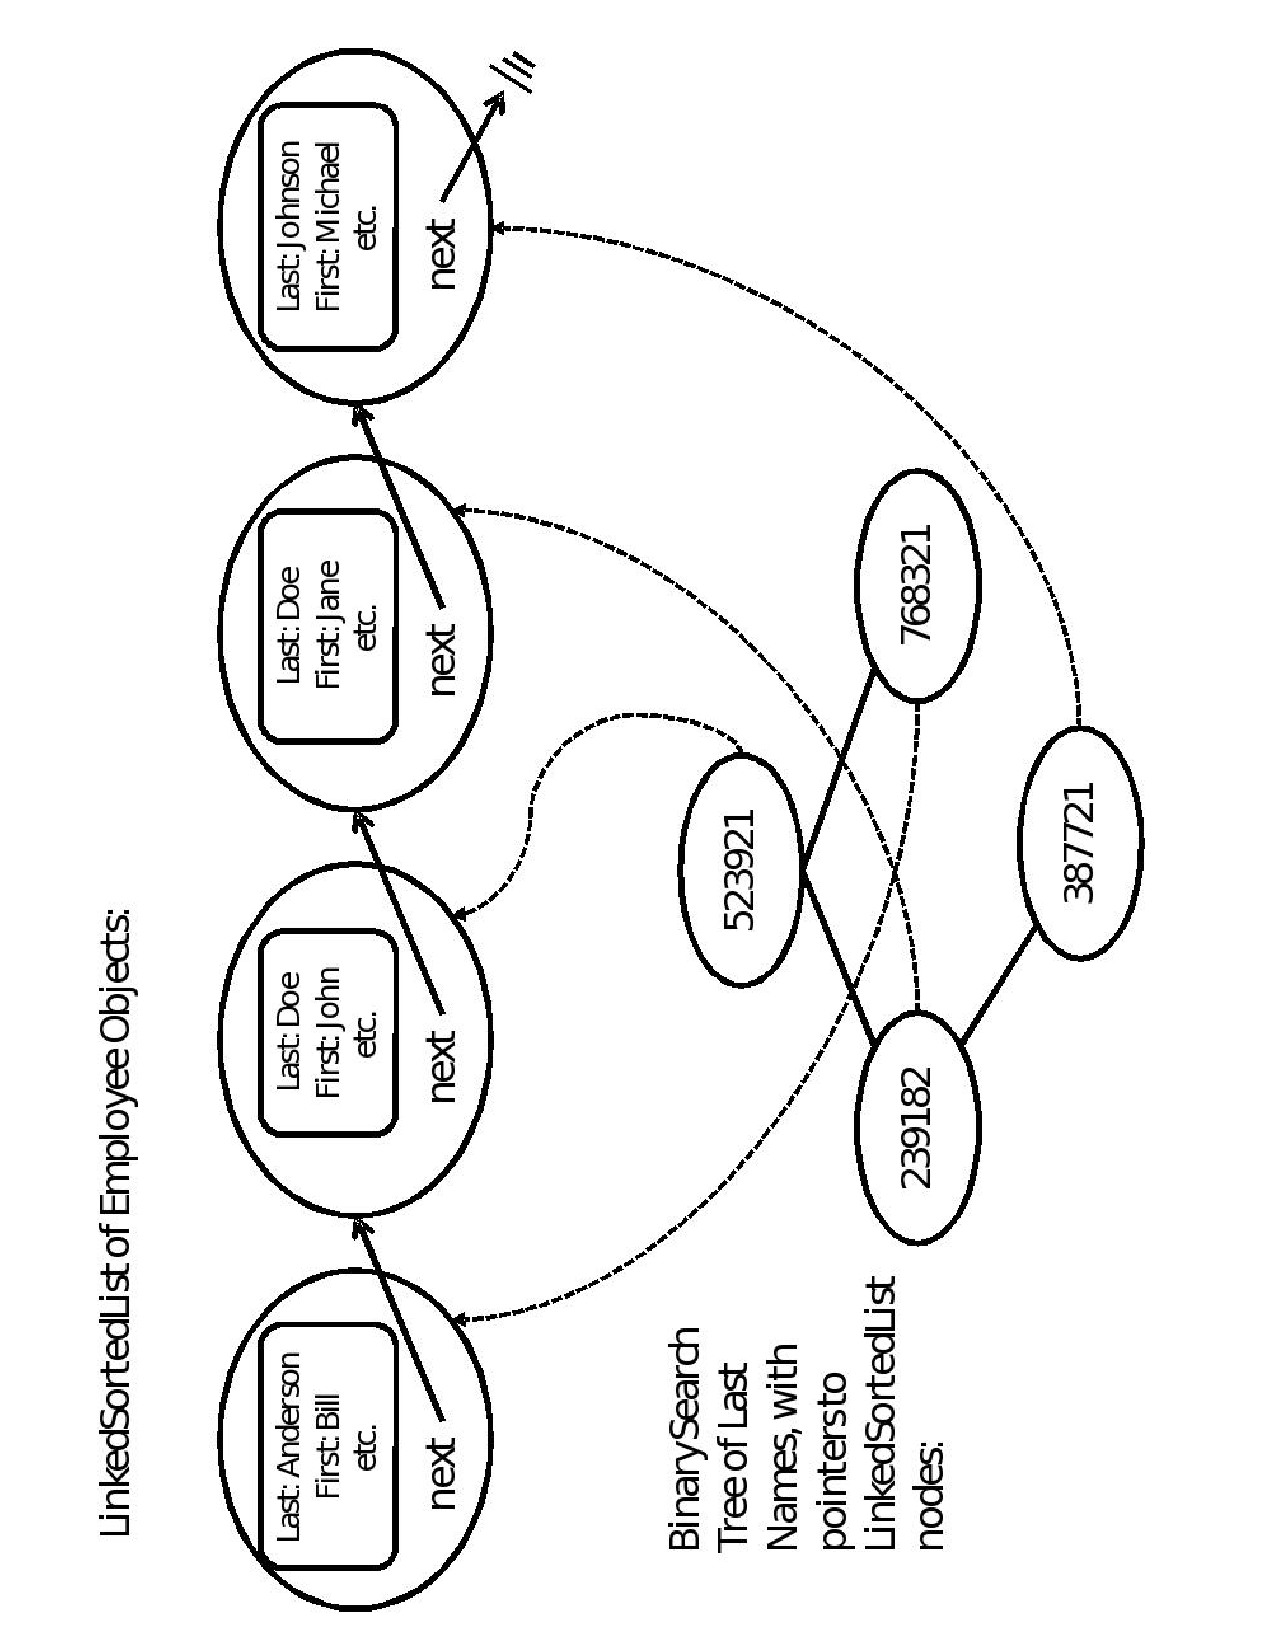
\includegraphics[scale=0.5,angle=-90]{structure.pdf}
  \caption{Structure of Linked Sorted List.\label{fig:list}}
  \vspace{-5pt}
\end{figure}

Your database should support the following operations:
\begin{itemize}
\item Insert new records (prompt user for all fields)
\item Search on Last Name (print ALL matching records)
\item Search on Employee ID (print matching record)
\item Delete records (by employee ID only)
\item Save database to disk (not including indexes)
\item Load database from disk (rebuilding indexes)
\end{itemize}

Saving the database should store records in last name order.  When
loading a database from the disk, all current records should be
deleted, and the database should be loaded from a file, and the
indexes should be rebuilt.  An example of a saved database file will
be provided – it will have the same format as the previous lab.  Your
program should be able to read this file and write files in this
format. \\

\textbf{The search operations should report the number of
tree nodes searched, in addition to the results.}  For example, an ID
query for 387721 would return results similar to the following:

\begin{verbatim}

MENU
(I)nsert new record
(D)elete record
(L)ast name search
(E)mployee ID search
(S)ave database to a file
(R)ead database from a file

 Enter choice: E

 Enter Employee ID:  387721
 Searching….

 3 index nodes searched.  Found 1 record:

 Last:  Johnson
 First: Michael
 EID:   387721
 Salary:$105,000
 Dept:  Legal
\end{verbatim}

\section{Requirements}
\begin{enumerate}
\item Your code should follow the Code Standards handed out during the
  first day of class.  Your code will be graded according to its
  correctness, efficiency, organization, and readability. 
\item Your main program should be called “lab3.cpp”.  You should implement
  your binary search tree in the files bst.h and bst.cpp. 
\item Make sure that each .cpp file includes your name in the header
  comments. 
\item Turn in all files needed to compile and execute your code (including
  any needed files from the previous lab) via webCT. If for some reason
  WebCT is unavailable, submit your source code by email tow lodarski.4
  AT wright.edu. If you want, you can also cc to the instructo r Meilin
  Liu, whose email address is meilin.liu AT wright.edu.   
\item If there are any special instructions that I need to know about, be
  sure to include a file named README.TXT in your lab2 directory
  detailing them. 
\item The grader will test your programs under the schools UNIX
  environment, e.g., unixapps1.wright.edu. It is YOUR responsibility
  to make your programs workable and runnable by others under school’s
  UNIX environment. 
\item The programming assignment is individual. You must do the project by
  yourself. If you allow others to copy your programs or answers, you
  will get the same punishment as those who copy yours. 
\end{enumerate}
\end{document}

%%%%%%%%%%%%%%%%%%%%%%%%%%%%%%%%%%%%%%%%%%%%%%%%%%%%%%%%%%%%%
